\documentclass[10pt,twocolumn,a4paper]{article}
\usepackage[margin=18mm,columnsep=7mm]{geometry}
\usepackage[T1]{fontenc}
\usepackage{lmodern}
\usepackage{amsmath,amssymb}
\usepackage{graphicx}
\usepackage{booktabs}
\usepackage{caption}
\usepackage[hidelinks]{hyperref}
\captionsetup{font=small,labelfont=bf}
\setlength{\emergencystretch}{2em}
\graphicspath{{../figures/}}
\renewcommand{\topfraction}{0.9}
\renewcommand{\dbltopfraction}{0.9}
\renewcommand{\textfraction}{0.07}
\renewcommand{\floatpagefraction}{0.85}
\renewcommand{\dblfloatpagefraction}{0.85}
\setcounter{dbltopnumber}{3}

\newcommand{\ket}[1]{\lvert #1\rangle}
\newcommand{\bra}[1]{\langle #1\rvert}
\newcommand{\proj}[1]{\ket{#1}\!\bra{#1}}

\title{Drawing the Mona Lisa with Quantum Supersampling}
\author{Rintaro Kanaji (6914500223)\thanks{Homework report for \emph{Programming Quantum
Computers}, Chapter~11.}}
\date{}

\begin{document}
\maketitle

\begin{abstract}
I apply Quantum Supersampling (QSS), introduced in Chapter~11 of
\emph{Programming Quantum Computers}, to a photograph of the Mona Lisa.
The painting is resized to $512\times512$ subpixels, converted to black and
white, and split into $128\times128$ tiles of $4\times4$ subpixels.
Each tile is written into the phases of a four-qubit register.
The number of white subpixels in the tile, which gives the brightness of one
output pixel, is then estimated with Grover iterations and an inverse quantum
Fourier transform (QFT).
I build the circuits in Qiskit, check them against theory, and compare QSS with
ordinary Monte Carlo sampling at the same cost.
In the book's setting (four counter qubits, one measurement per tile), QSS
lowers the average pixel error by $21\%$ and almost doubles the fraction of
exactly correct pixels ($50.8\%$ versus $28.6\%$).
The errors that remain are fewer but larger. This reproduces the book's main
message: a quantum computer can change the \emph{character} of the noise.
\end{abstract}

%-------------------------------------------------------------------------
\section{Introduction}

In computer graphics, each pixel of an image is often computed as the average of
many samples. This is called \emph{supersampling}, or Monte Carlo sampling.
Only the \emph{sum} of the samples is needed, not each sample itself.
Chapter~11 of the textbook~\cite{pqc} shows that a quantum computer can estimate
such a sum directly. The method is called Quantum Supersampling (QSS). It is not
faster than Monte Carlo sampling, but its errors look different: many pixels
come out exactly right, and the rest can be badly wrong.

The book tests QSS on simple shapes such as lines and circles.
In this report I apply it to a photograph, the Mona Lisa.
Section~\ref{sec:methods} introduces the methods,
Sections~\ref{sec:prep}--\ref{sec:qss} explain how they are applied,
Section~\ref{sec:impl} describes the implementation, and
Sections~\ref{sec:results}--\ref{sec:disc} present and discuss the results.

%-------------------------------------------------------------------------
\section{Methods}\label{sec:methods}

Table~\ref{tab:methods} lists the methods used and their roles.

\begin{table}[t]
\centering\small
\caption{Methods used in this work.}
\label{tab:methods}
\begin{tabular}{ll}
\toprule
Method & Role in this work\\
\midrule
Superposition (H gates) & blank canvas\\
Phase encoding (oracle) & draw one tile\\
Amplitude amplification & Grover iteration\\
Inverse QFT & read the result\\
Quantum sum estimation & count white subpixels\\
QSS lookup table & readout $\to$ brightness\\
Bitplanes & colour image\\
Monte Carlo sampling & comparison\\
Bayer dithering & grey $\to$ black/white\\
\bottomrule
\end{tabular}
\end{table}

\paragraph{Phase encoding.}
Hadamard gates put a register into an equal superposition of all its basis
states. Each basis state stands for one pixel; this is the ``blank canvas''.
A pixel is coloured white by flipping the sign (phase $\pi$) of its basis state.
The operation that does this for all white pixels is called a \emph{phase
oracle}.

\paragraph{Amplitude amplification.}
A Grover iteration applies the oracle and then a reflection (the book's
\texttt{mirror}). Repeating it makes the probability of the white pixels
oscillate, and the speed of this oscillation depends on \emph{how many} pixels
are white.

\paragraph{Inverse QFT.}
The inverse QFT reads out the frequency of such an oscillation, in the same way
a Fourier transform finds the frequency of a signal.

\paragraph{Quantum sum estimation.}
Combining the two gives the number of white pixels without reading any single
pixel. This is the book's ``Multiple Flipped Entries'' example, also known as
quantum counting~\cite{brassard}. QSS uses it once per tile.

\paragraph{Lookup table.}
The measured number is only statistically related to the count. A table,
computed once in advance, converts each measured value into the most likely
count.

\paragraph{Classical parts.}
Bayer dithering turns grey levels into black-and-white patterns. Bitplanes
treat the red, green and blue channels as three separate black-and-white
images. Monte Carlo sampling, which estimates brightness from randomly chosen
subpixels, is used for comparison.

\paragraph{Tools.}
Circuits are built and simulated with Qiskit~2.6 (exact statevector
simulation). NumPy, SciPy, Pillow and Matplotlib are used for image processing
and figures. Circuit diagrams are drawn with Qiskit, and circle-notation views
of quantum states are taken from the book's QCEngine simulator so that they
look the same as in the book.

%-------------------------------------------------------------------------
\section{Image preparation}\label{sec:prep}

The input image ($408\times530$) is cropped to a square, keeping the head, and
resized to $512\times512$.
It is then converted to black and white with a $4\times4$ Bayer pattern that is
aligned with the tiles (Fig.~\ref{fig:prep}).
With this pattern, a tile with grey level $g$ contains about $16g$ white
subpixels. The \emph{ideal} brightness of an output pixel is therefore
\begin{equation}
L^{\star}=\frac{k}{16},
\label{eq:ideal}
\end{equation}
where $k\in\{0,\dots,16\}$ is the number of white subpixels in its tile.
For colour, the red, green and blue channels are converted separately.

\begin{figure*}[t]
\centering
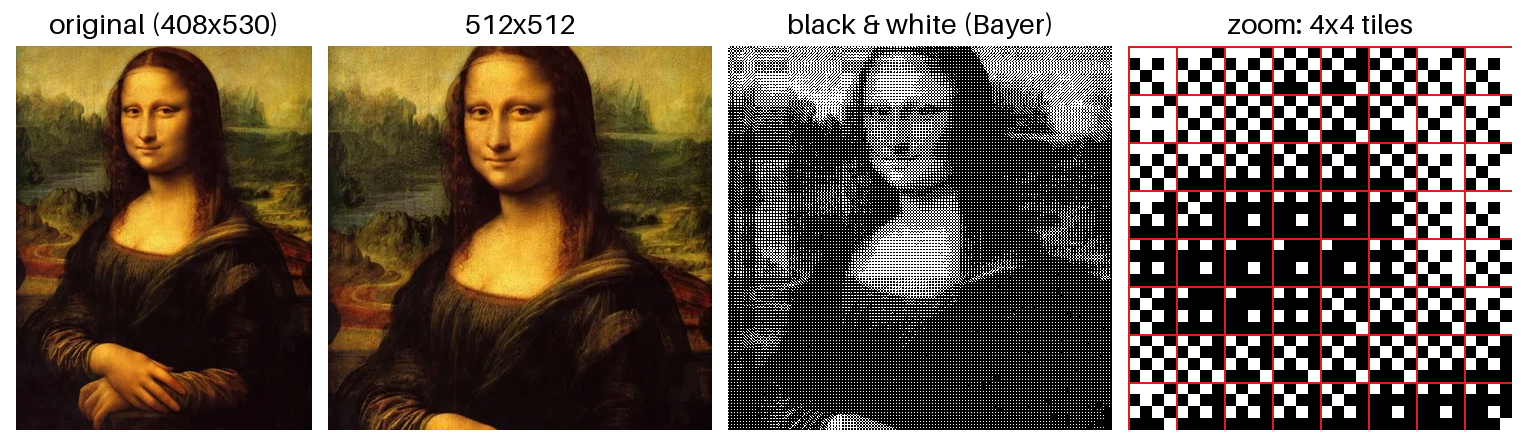
\includegraphics[width=\textwidth]{step1_overview.png}
\caption{Image preparation. From left: original, $512\times512$ crop,
black-and-white image (white $=$ phase $\pi$), and a zoom with the $4\times4$
tile grid in red. Each tile becomes one output pixel.}
\label{fig:prep}
\end{figure*}

%-------------------------------------------------------------------------
\section{Drawing a tile}\label{sec:encode}

The 16 subpixels of a tile are numbered $x=4q_y+q_x\in\{0,\dots,15\}$, where
$q_x$ and $q_y$ (each $0$--$3$) are the column and row inside the tile, and are
stored in four qubits (two for $q_x$, two for $q_y$). Let $f(x)=1$ if subpixel $x$ is white and $0$ otherwise.
Hadamard gates create the blank canvas, and the oracle flips the sign of the
white subpixels:
\begin{equation}
\frac14\sum_{x=0}^{15}\ket{x}
\;\xrightarrow{\;O_f\;}\;
\frac14\sum_{x=0}^{15}(-1)^{f(x)}\ket{x}.
\label{eq:encode}
\end{equation}
All 16 amplitudes keep the same size; the picture is stored only in the signs
(Fig.~\ref{fig:circle}).
The book draws shapes with arithmetic, but a photograph has no simple formula.
I therefore flip each white subpixel separately, using one multi-controlled $Z$
gate per white subpixel, with $X$ gates to select the subpixel.

\begin{figure}[t]
\centering
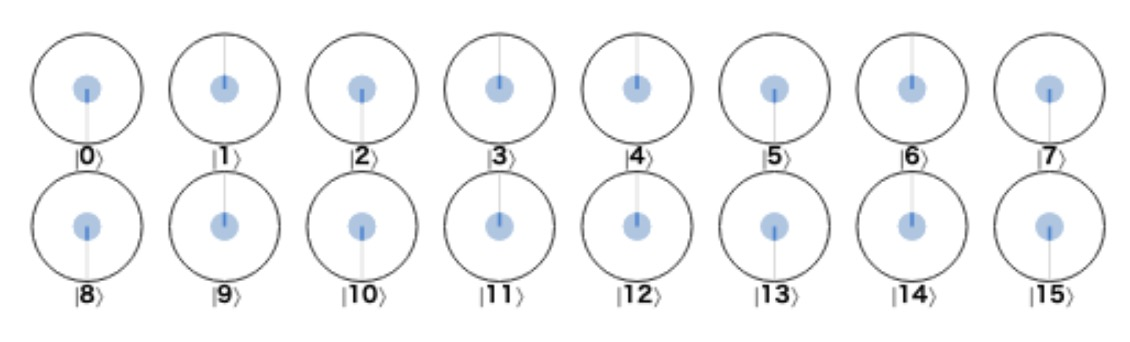
\includegraphics[width=\columnwidth]{circle_notation_qcengine.jpg}
\caption{Circle notation of one tile (row~35, column~64; a checkerboard with
$k=8$) after phase encoding, produced with the book's QCEngine simulator. The
circle for basis state $\ket{x}$ is subpixel $x=4q_y+q_x$. Line up: phase $0$
(black). Line down: phase $\pi$ (white).}
\label{fig:circle}
\end{figure}

%-------------------------------------------------------------------------
\section{Counting the white subpixels}\label{sec:qss}

\subsection{Grover iteration}
One Grover iteration is the oracle followed by the book's \texttt{mirror}:
\begin{equation}
Q=\bigl(I-2\proj{s}\bigr)\,O_f ,
\label{eq:Q}
\end{equation}
where $\ket{s}$ is the blank canvas. Define the angle $\theta$ by
\begin{equation}
\sin^2\theta=\frac{k}{16}.
\label{eq:theta}
\end{equation}
Each application of $Q$ rotates the state by the angle $2\theta$. Counting the
white subpixels therefore means measuring $\theta$.

\subsection{Counter register and inverse QFT}
A counter of $t$ qubits (so $N=2^t$ possible values) decides how many times $Q$
is applied: counter qubit $j$ controls $Q^{2^j}$ (Fig.~\ref{fig:qss}).
Because the counter is in superposition, all repetition counts
$0,1,\dots,N-1$ are run at once. The inverse QFT then turns the rotation
speed into a measured number $y\in\{0,\dots,N-1\}$, which lands close to
\begin{equation}
y\approx N\left(\frac12\pm\frac{\theta}{\pi}\right).
\label{eq:peak}
\end{equation}
For example, a black tile ($k=0$) gives $y\approx N/2$ and a white tile
($k=16$) gives $y\approx0$. Because of the ``$\pm$'', the readouts $y$ and $N-y$
mean the same brightness.

\subsection{Lookup table}
The measured $y$ is spread around Eq.~\eqref{eq:peak}, so I compute the
probability $P(y\mid k)$ of every readout $y$ for every count $k$ once, from
the circuit itself (Fig.~\ref{fig:lut}; book Example~11-5). A measurement is
decoded to the most likely count, as in book Example~11-4:
\begin{equation}
\hat k=\text{the $k$ with the largest }P(y\mid k),\qquad \hat L=\hat k/16 .
\label{eq:decode}
\end{equation}
The same table also gives a \emph{confidence}: how likely it is that $\hat k$ is
correct, given $y$.

With $t=4$ there are only 16 readouts, and $y$ and $N-y$ mean the same thing.
Only nine counts can therefore be output, $\hat k\in\{0,1,2,5,8,11,14,15,16\}$
(out of 17). With $t=6$ all 17 levels can be output.

\begin{figure}[t]
\centering
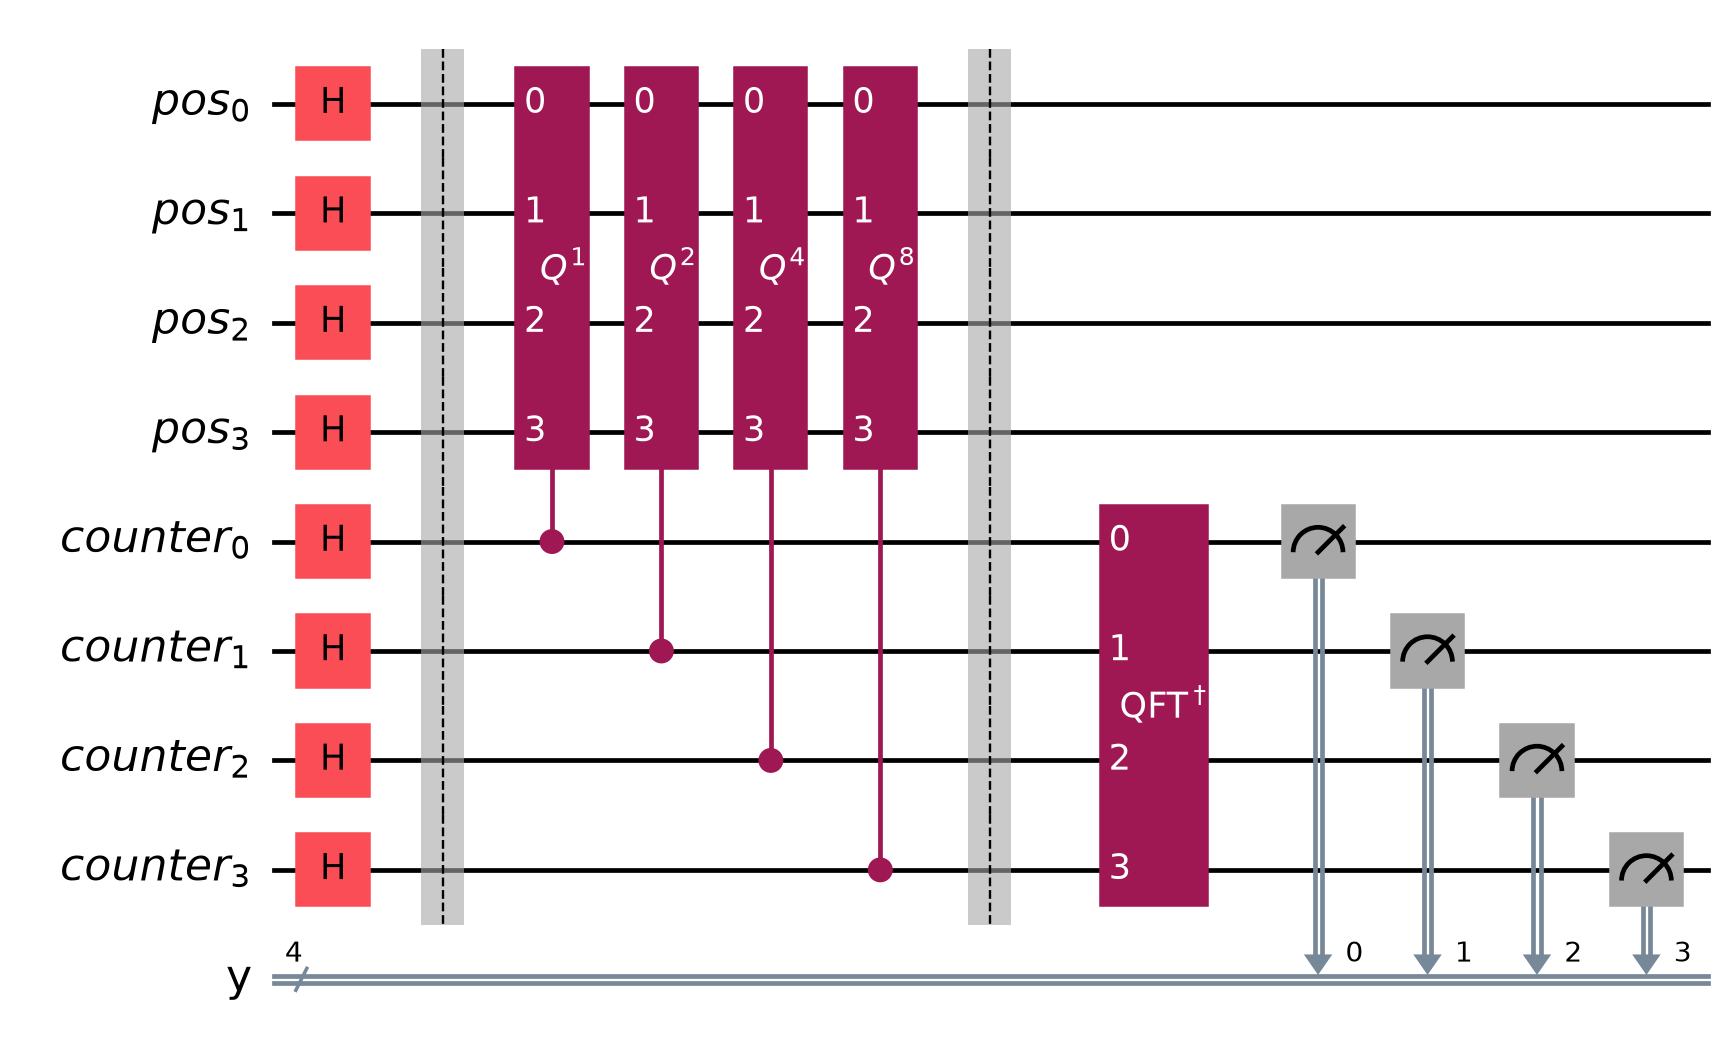
\includegraphics[width=\columnwidth]{circuit_qss_overview_t4.png}
\caption{QSS circuit for one tile ($t=4$). Counter qubit $c_j$ controls
$Q^{2^j}$; the inverse QFT turns the counter into the readout $y$.}
\label{fig:qss}
\end{figure}

\begin{figure*}[t]
\centering
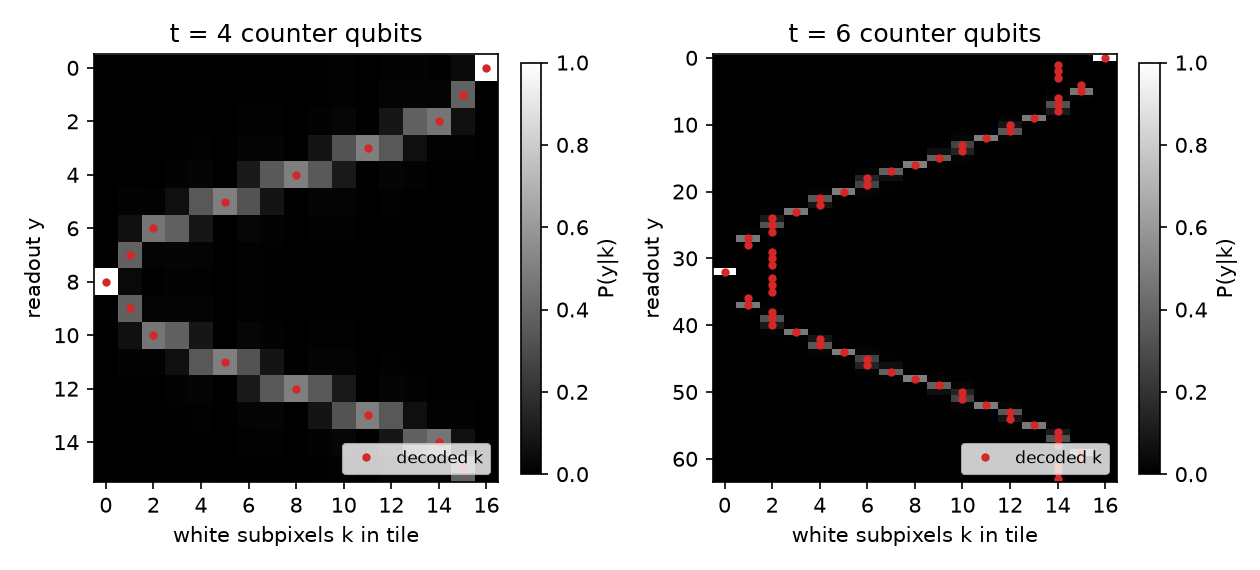
\includegraphics[width=0.6\textwidth]{lookup_tables.png}
\caption{QSS lookup tables $P(y\mid k)$ for $t=4$ (left) and $t=6$ (right)
counter qubits. Bright cells are likely readouts; red dots show the decoded
count. Compare book Figs.~11-14 and 11-16.}
\label{fig:lut}
\end{figure*}

\subsection{Circuits}
Figure~\ref{fig:qss} shows the whole circuit for one tile with $t=4$
(8 qubits). Figure~\ref{fig:grover} shows one controlled Grover iteration
gate by gate. Only the multi-controlled $Z$ gates need the extra counter
control; the $X$ and $H$ gates around them cancel when the counter qubit is
$\ket0$, as in the book's \texttt{mask\_with\_condition}.
Figure~\ref{fig:iqft} shows the inverse QFT.

\begin{figure*}[t]
\centering
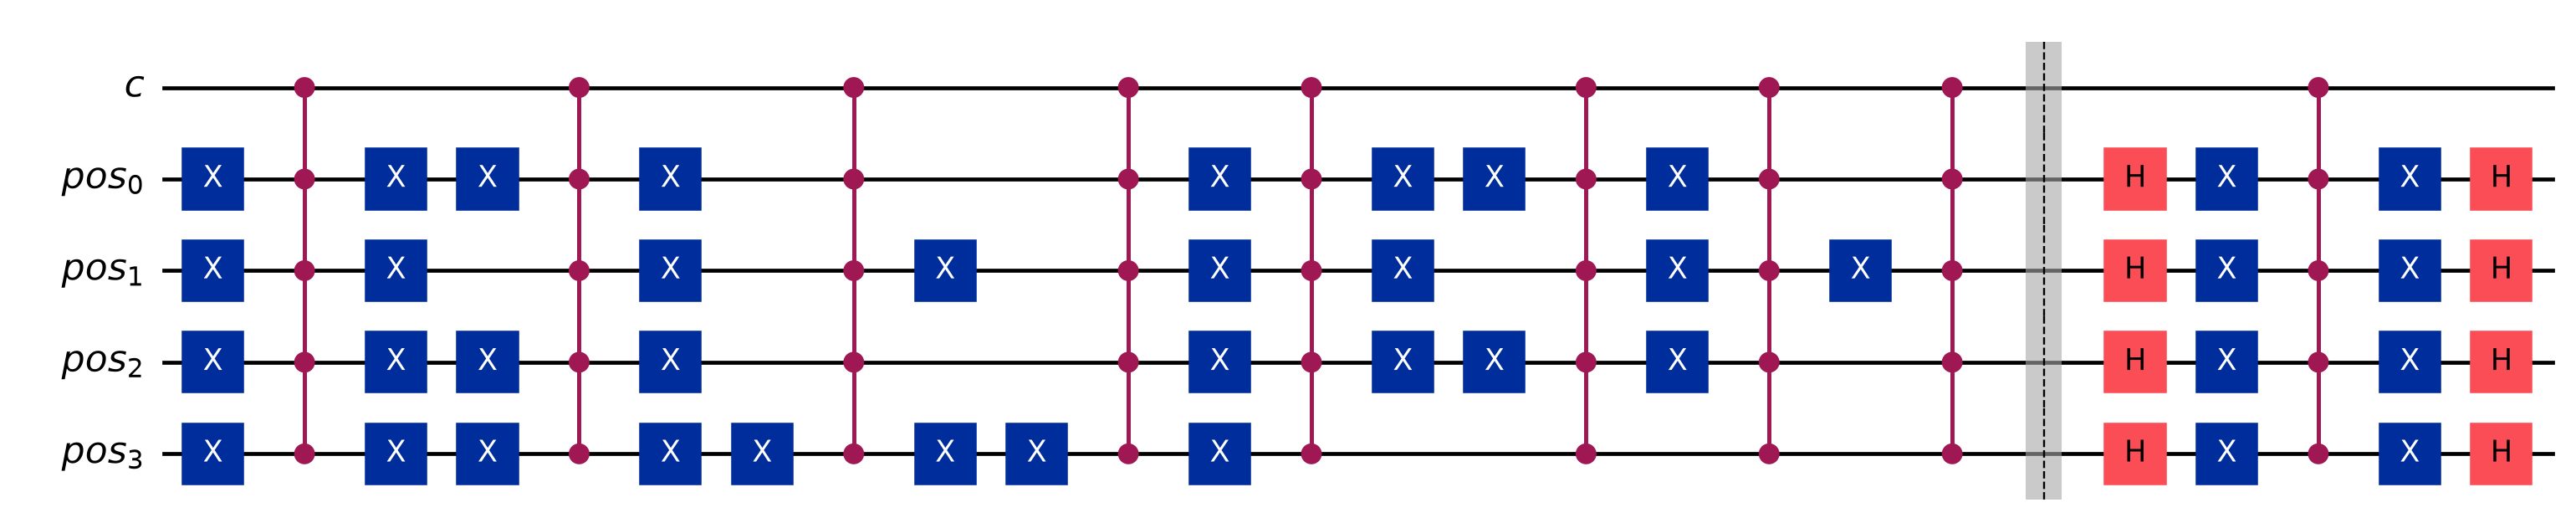
\includegraphics[width=\textwidth]{circuit_grover_step_controlled.png}
\caption{One controlled Grover iteration for the tile of Fig.~\ref{fig:circle}.
Left of the barrier: the oracle (eight phase flips, one per white subpixel).
Right: the \texttt{mirror}. Only the multi-controlled $Z$ gates carry the counter
control $c$.}
\label{fig:grover}
\end{figure*}

\begin{figure}[t]
\centering
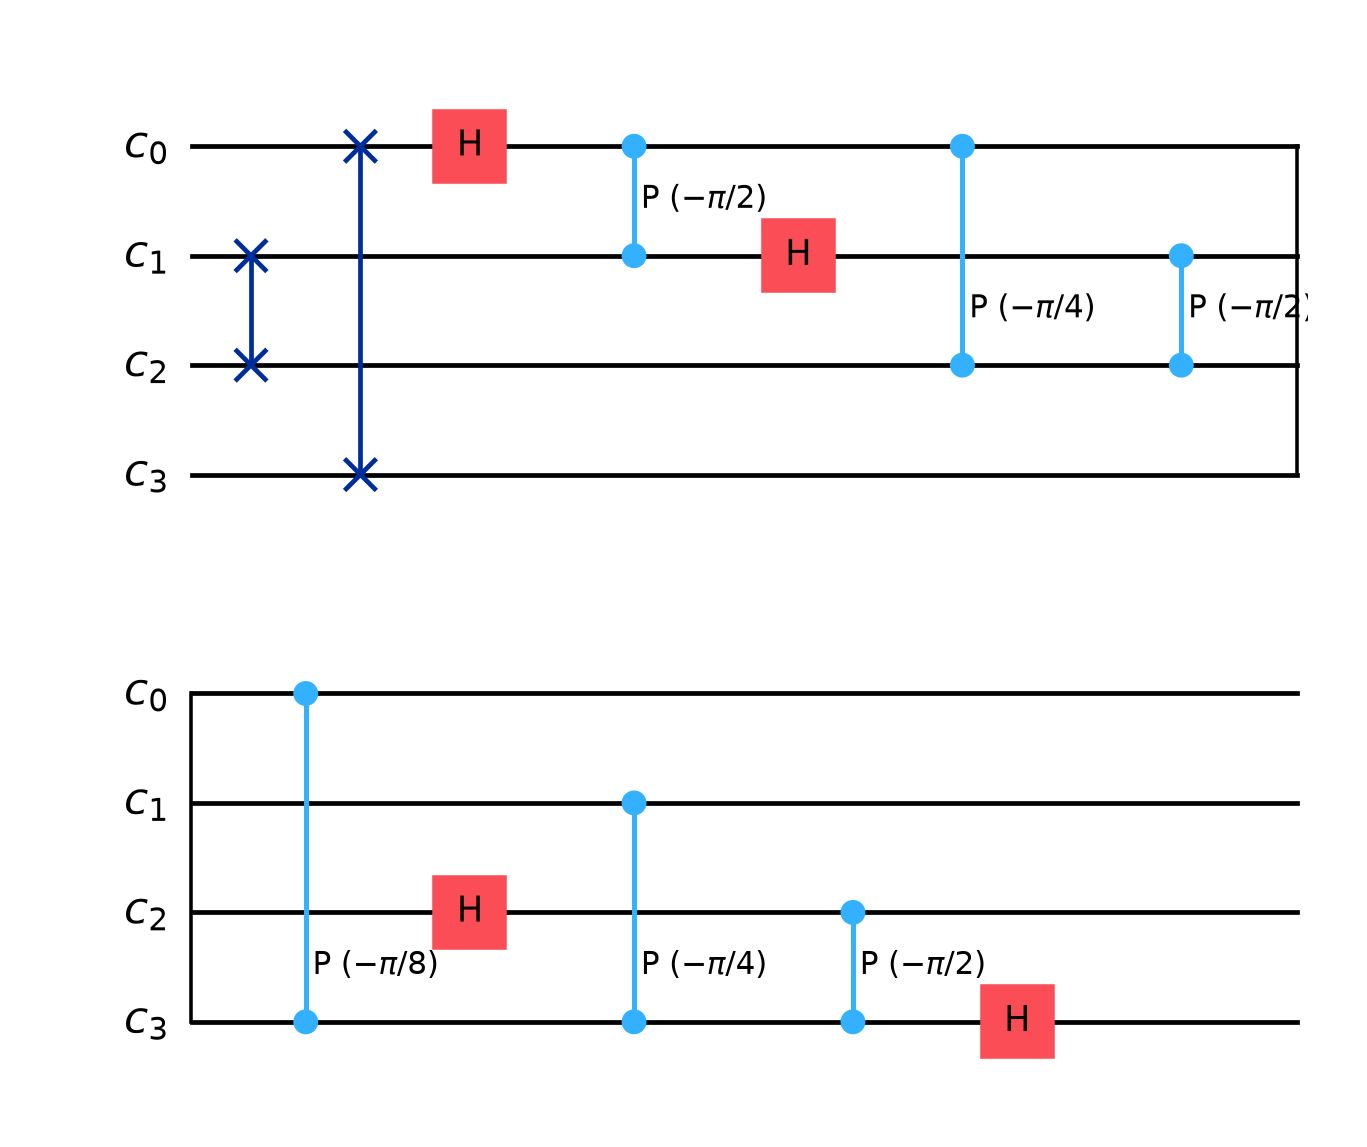
\includegraphics[width=0.85\columnwidth]{circuit_inverse_qft_t4.png}
\caption{Four-qubit inverse QFT: SWAP gates, Hadamard gates and controlled
phase gates.}
\label{fig:iqft}
\end{figure}

%-------------------------------------------------------------------------
\begin{figure*}[t]
\centering
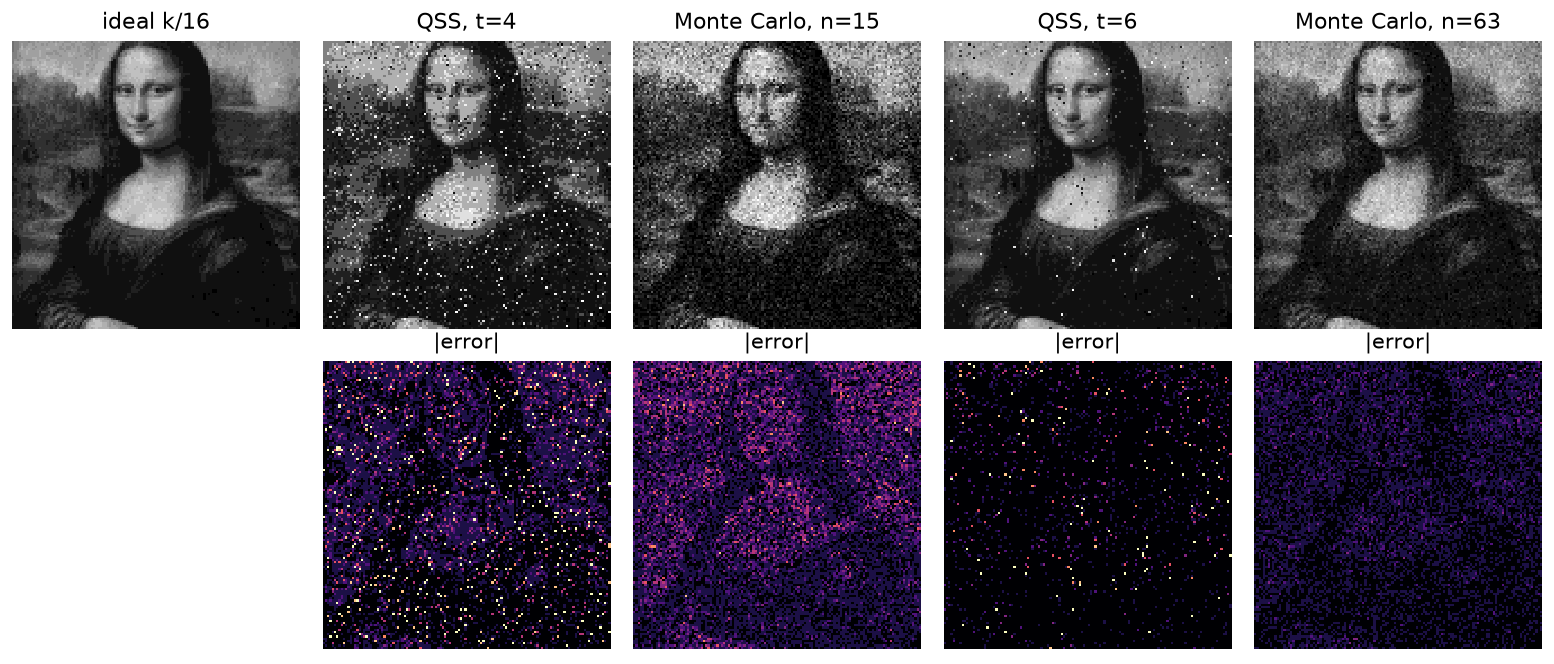
\includegraphics[width=0.88\textwidth]{comparison_gray.png}
\caption{Greyscale results ($128\times128$). Top, from left: ideal; QSS
($t=4$); Monte Carlo ($n=15$); QSS ($t=6$); Monte Carlo ($n=63$). Bottom: the
error of each pixel (bright $=$ large error).}
\label{fig:gray}
\end{figure*}

\begin{figure*}[t]
\centering
\begin{minipage}[b]{0.56\textwidth}
\centering
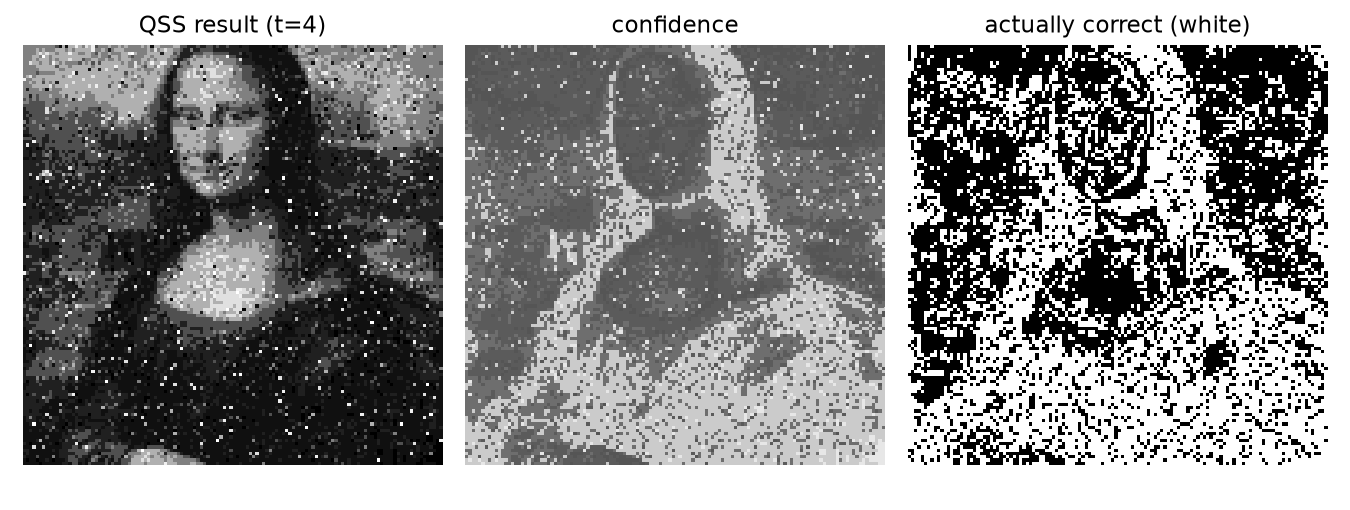
\includegraphics[width=\linewidth]{confidence_t4.png}
\caption{QSS result ($t=4$), its confidence map (bright $=$ likely correct),
and the pixels that are actually correct (white).}
\label{fig:conf}
\end{minipage}\hfill
\begin{minipage}[b]{0.40\textwidth}
\centering
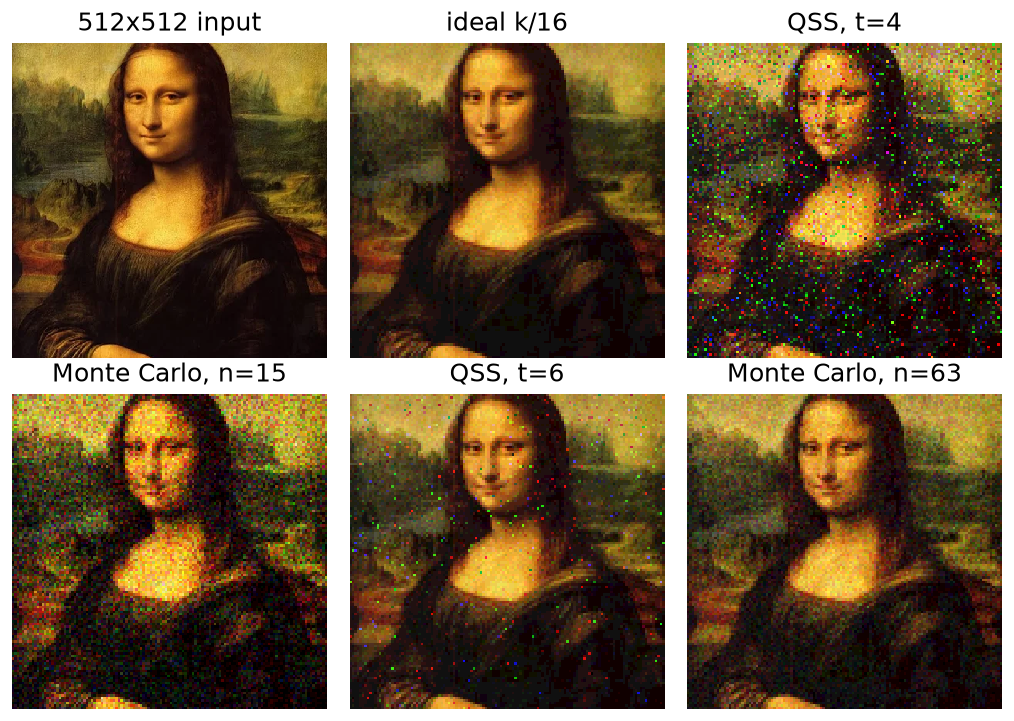
\includegraphics[width=\linewidth]{comparison_rgb.png}
\caption{Colour by bitplanes. Top: input, ideal, QSS ($t=4$). Bottom: Monte
Carlo ($n=15$), QSS ($t=6$), Monte Carlo ($n=63$).}
\label{fig:rgb}
\end{minipage}
\end{figure*}

\section{Implementation and checks}\label{sec:impl}

All circuits are built from basic Qiskit gates and simulated exactly.
I checked that
(a)~the circuit of one Grover iteration equals Eq.~\eqref{eq:Q} as a matrix,
(b)~moving the white subpixels around inside a tile does not change the
readout probabilities,
(c)~40 real tiles of the Mona Lisa give the lookup-table column for their own
$k$, and
(d)~the simulated table agrees with the theoretical formula for phase
estimation.
All four checks agree to within $10^{-11}$ or better.

Because of (b) and (c), the readout of a tile depends only on its count $k$.
To render all $16\,384$ tiles quickly, I therefore draw one readout per tile
directly from the lookup table. This gives the same statistics as running each
tile's circuit once.

\subsection{Monte Carlo comparison}
Ordinary supersampling looks at $n$ randomly chosen subpixels and reports the
fraction that are white, rounded to the same 17 levels. Its typical error is
\begin{equation}
\sigma_{\mathrm{MC}}=\sqrt{\frac{p(1-p)}{n}},\qquad p=\frac{k}{16},
\label{eq:mc}
\end{equation}
which shrinks like $1/\sqrt n$. The QSS circuit calls the oracle
$1+2+\dots+2^{t-1}=2^t-1$ times, so for a fair comparison I use $n=2^t-1$, that
is, $n=15$ for $t=4$ and $n=63$ for $t=6$. The QSS error shrinks faster, like
$1/N$, which is the usual advantage of amplitude estimation~\cite{brassard}.

Note that a tile has only 16 subpixels, so a classical program could simply
read all of them. As in the book, the comparison is made at a fixed sample
budget, as in a real renderer, where the number of possible samples is huge.

%-------------------------------------------------------------------------
\section{Results}\label{sec:results}

I measure two things: the mean absolute error (MAE) between the result and the
ideal image of Eq.~\eqref{eq:ideal}, and the fraction of pixels that are
exactly correct. Table~\ref{tab:gray} shows the results. The numbers in
parentheses are the values predicted from the lookup table, and they agree well
with the simulation.

\begin{table}[t]
\centering\small
\setlength{\tabcolsep}{4pt}
\caption{Greyscale results at the same number of oracle calls per pixel.
Predicted values in parentheses.}
\label{tab:gray}
\begin{tabular}{lccc}
\toprule
Method & Calls & MAE & Exact (\%)\\
\midrule
QSS, $t=4$ & 15 & \textbf{0.0574} (0.0591) & \textbf{50.8} (50.5)\\
Monte Carlo & 15 & 0.0725 (0.0725) & 28.6 (28.1)\\
\midrule
QSS, $t=6$ & 63 & \textbf{0.0115} (0.0109) & \textbf{91.1} (91.2)\\
Monte Carlo & 63 & 0.0321 (0.0322) & 54.6 (54.3)\\
\bottomrule
\end{tabular}
\end{table}

\paragraph{Error level.}
In the book's setting ($t=4$), QSS lowers the MAE by $21\%$ and gives
$1.78\times$ as many exact pixels. The book reports about $33\%$ and about
$2\times$ for its own test image, so the trend is the same. At $t=6$, QSS lowers
the MAE by $64\%$, with $91.1\%$ of pixels exactly correct against $54.6\%$
for Monte Carlo.

\paragraph{Character of the noise.}
The error maps in Fig.~\ref{fig:gray} show the effect described in the book.
Monte Carlo makes a small error on most pixels, like fine grain.
QSS gets more pixels exactly right (about half at $t=4$, $91\%$ at $t=6$) and
makes fewer but larger mistakes. At
$t=4$ some of these come from the levels that cannot be output (Sec.~\ref{sec:qss}).
At $t=6$ only $8.9\%$ of pixels are wrong, and these appear as isolated specks.
In the book's words, Monte Carlo \emph{converges toward} the right answer,
while QSS increases the \emph{probability} of getting exactly the right answer.
Isolated specks are also easy to clean up afterwards, for example with a median
filter; fine grain is not.

\paragraph{Confidence map.}
Figure~\ref{fig:conf} shows the confidence of each QSS pixel, computed only
from the measured values. Confidence is high for very dark and very bright
pixels and low for mid-tones, and it matches the pixels that are actually
correct reasonably well (correlation $0.47$). It could be used to re-measure
only the doubtful pixels.

\paragraph{Colour.}
Following the book's ``Adding Color'' section, the red, green and blue images
are processed separately and recombined (Fig.~\ref{fig:rgb}). With 17 levels per
channel this gives $17^3=4913$ colours, about the ``12-bit'' image of the book.
At $t=4$, QSS has an MAE of $0.050$ with $58.7\%$ exact values, against $0.064$
and $34.0\%$ for Monte Carlo. A QSS error appears as a single red, green or blue
speck, because only one channel is wrong.

%-------------------------------------------------------------------------
\section{Discussion}\label{sec:disc}

\paragraph{What the quantum computer adds.}
QSS never reads an individual subpixel; it estimates the total number of white
subpixels in one go. The oracle is still called $2^t-1$ times per pixel, so it
is not faster. The benefit is the different shape of the error.

\paragraph{Why $t=4$ is limited.}
With four counter qubits only nine of the 17 brightness levels can be output,
and mid-tones such as $k=8$ and $k=9$ give almost the same readout. This
explains the lower accuracy and confidence at mid-tones. Both problems
disappear at $t=6$.

\paragraph{Cost of drawing a photograph.}
The book's shapes need only a few arithmetic gates. A photograph needs one
multi-controlled gate per white subpixel, so one tile already needs thousands
of two-qubit gates. This is far beyond today's noisy hardware. Smarter oracle
construction could reduce the cost.

\paragraph{Other ways to store images.}
Methods such as FRQI~\cite{frqi} and NEQR~\cite{neqr} store grey levels
directly. As the book explains, however, storing brightness in the amplitudes
would break the counting that QSS relies on. QSS therefore keeps a
black-and-white phase image and obtains grey levels by dithering.

\paragraph{Limitations.}
All results come from noiseless simulation, and the image is prepared on a
classical computer. The results show how the algorithm behaves; they do not
show an advantage on real hardware.

%-------------------------------------------------------------------------
\section{Conclusion}
I drew the Mona Lisa with the QSS method of Chapter~11. The method uses phase
encoding, Grover iterations, an inverse QFT, a lookup table and colour
bitplanes. At the same cost, QSS gives a smaller average error than Monte Carlo
and nearly twice as many exactly correct pixels, and its errors take the form of
a few larger mistakes instead of grain on every pixel. This reproduces the
book's main point: a quantum computer can be useful by changing the noise, even
without being faster.

\section*{Code availability}
The code and results are available at
\url{https://github.com/kanaji2002/Quantum-homework-2}.
\texttt{src/prepare\_image.py} prepares the image, and \texttt{src/qss.py}
builds the circuits, runs the checks and draws all figures.

\begin{thebibliography}{9}\small
\bibitem{pqc} E.~R.~Johnston, N.~Harrigan, M.~Gimeno-Segovia,
\emph{Programming Quantum Computers}, O'Reilly, 2019, Ch.~11.
\bibitem{brassard} G.~Brassard, P.~H{\o}yer, M.~Mosca, A.~Tapp, ``Quantum
amplitude amplification and estimation,'' \emph{Contemp.\ Math.}\
\textbf{305}, 53--74 (2002).
\bibitem{frqi} P.~Q.~Le, F.~Dong, K.~Hirota, ``A flexible representation of
quantum images,'' \emph{Quantum Inf.\ Process.}\ \textbf{10}, 63--84 (2011).
\bibitem{neqr} Y.~Zhang, K.~Lu, Y.~Gao, M.~Wang, ``NEQR: a novel enhanced
quantum representation of digital images,'' \emph{Quantum Inf.\ Process.}\
\textbf{12}, 2833--2860 (2013).
\end{thebibliography}

\end{document}
